\thispagestyle{empty}
\Large
\begin{center}
\Huge\bfseries Hochfrequenzuntersuchungen an\\
zweidimensionalen Elektronensystemen\\
auf dünnen Heliumfilmen
\end{center}
\vspace{1ex}
\begin{center}
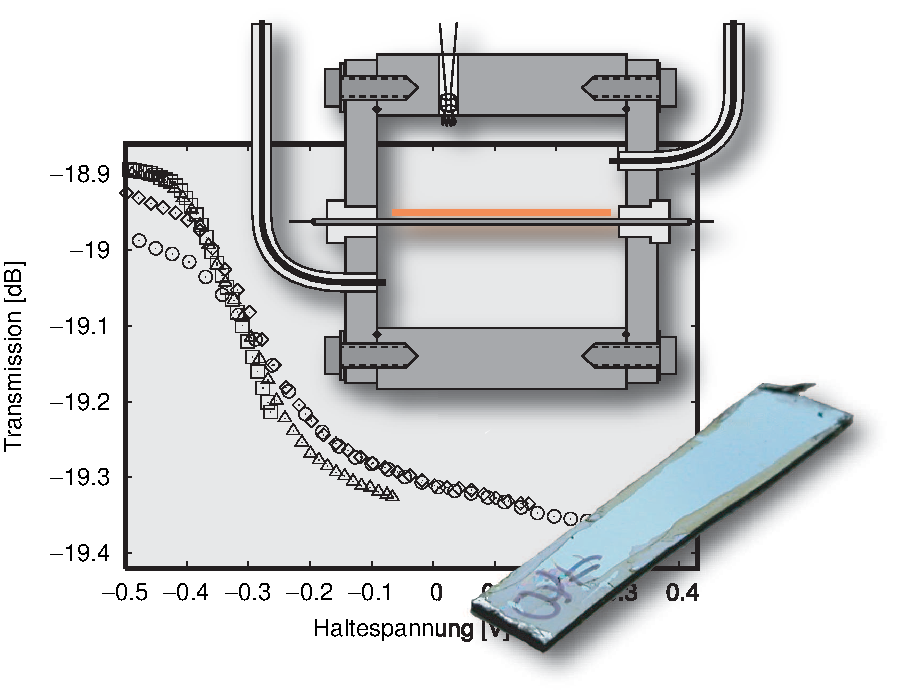
\includegraphics[width=8cm]{titel/titelbild}
\end{center}
\vspace{2ex}
\begin{center}
\LARGE\bfseries Dissertation
\end{center}
\vspace{2ex}
\centerline{zur Erlangung des akademischen Grades}
\centerline{des Doktors der Naturwissenschaften}
\vspace{4ex}
\centerline{an der Universität Konstanz,}
\centerline{Mathematisch-Naturwissenschaftliche Sektion,}
\centerline{Fachbereich Physik}
\vspace{4ex}
%centerline{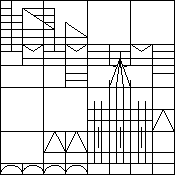
\includegraphics[width=2cm]{titel/unilogo}}
%\vspace{2ex}
\centerline{vorgelegt von}
\vspace{2ex}
\centerline{\bfseries Andreas Würl}
\vspace{5ex}
\centerline{Tag der mündlichen Prüfung: 24.~Juli 2006}
\vspace{0.5ex}
\centerline{\begin{tabular}{l}
Referent: Prof.~Dr.~Paul~Leiderer\\
Referent: Prof.~Dr.~Elke~Scheer
\end{tabular}}
\normalsize
\newpage
\mbox{}\thispagestyle{empty}
\newpage
\setcounter{page}{1}
